\chapter{Entwurf} \label{chp:design}

\section{Anforderungsanalyse} \label{sec:requirements} Die Anforderungsanalyse 
eines Systems oder Programms besteht aus den Beschreibungen der zu leistenden Funktionen und 
den bestehenden Beschränkungen, welchen das System unterliegt.
Dabei wird in \textit{Benutzeranforderungen} und \textit{Systemanforderungen} unterschieden. 
Ersteres wird dabei in Diagrammen und Listen dargestellt, während letzteres eine detailliertere Beschreibung der Software-Funktionen umfasst \cite{Sommerville.2016}. In diesem Zusammenhang werden zunächst grobe Anforderungen gesammelt, um anschließend eine genauere Beschreibung darzulegen. \\
Die Anforderungen werden zudem in funktionale und nicht-funktionale Anforderungen unterteilt \cite{Sommerville.2016}:
\begin{itemize}
    \item \textit{Funktionale Anforderungen} stehen für das Verhalten der Software auf zum Beispiel Benutzereingaben oder in diesem Fall Abfragen an einen Server 
    \item \textit{Nicht-funktionale Anforderungen} sind beispielsweise Beschränkungen, welche durch bestehende Standards entstehen. 
\end{itemize}
Daraus lässt sich schließen, dass funktionale Anforderungen direkt mit der Funktion des Systems in Verbindung gebracht werden können, während nicht funktionale Anforderungen die technischen Einschränkungen beschreiben. Die folgende Tabelle illustriert die Benutzeranforderungen und teilt sie in die aufgezeigten Sparten ein:

\begin{table}[ht]
    \begin{tabular}{@{}ll@{}}
    \toprule
    \textbf{Funktional} & \textbf{Nicht-funktional} \\ 
        \midrule
    \begin{tabular}[c]{@{}l@{}}Oberfläche zur Konfiguration der \gls{restapi}\\
            \tabitem Manuelles Hinzufügen von Ressourcen \\
            \tabitem Hinzufügen von Ressourcen durch \\ \gls{csv} Datei\\
            \tabitem Visuelle Darstellung der Endpunkte \\
    \end{tabular} & 
    \begin{tabular}[c]{@{}l@{}}
        Betriebssystemunabhängiges Ausführen\\ 
        der Software
    \end{tabular} \\ 
        \midrule
        Persistente Datenspeicherung 
        & Operiert ohne Internetverbindung \\ 
        \midrule
        & \textit{REST}-Konform\\ 
        \bottomrule
    \end{tabular}
    \caption{Benutzeranforderungen}
\end{table}
\newpage
\subsection*{Systemanforderungen} \label{subsec:systemrequirements}
Das System muss auf den bekannten Betriebssystemen \textit{Windows}, \textit{Mac OS} sowie \textit{Linux} lauffähig sein und ohne Internetverbindung gestartet, genutzt und konfiguriert werden können. Das Starten des Programms führt zur ausführung eines Servers, welcher die \gls{api} und die Benutzeroberfläche bereitstellt. Des Weiteren muss das System \gls{rest}-Komform sein. Dies bedeutet, es unterliegt einer Reihe von inoffiziellen Regeln bzw. \textit{Best-Practises}, welche im Folgenden aufgelistet werden \cite{Masse.2012}:

\paragraph{Request Methoden}
Abfragen oder auch \textit{Requests} werden normgerecht verwendet. Es gibt gewisse Semantiken, die hier Verwendung finden und nach dem \gls{crud} Prinzip auf die \gls{restapi} angewendet werden.  \cite{nwg.1999} \cite{Masse.2012}:

\begin{itemize}
    \item \textbf{GET} Anzeigen von Ressourcen; wobei ohne Parameter alle Einträge abgerufen werden. (Read) \\
    Beispiel: \textit{GET http://api.localhost/studenten} \\
    Beispiel: \textit{GET http://api.localhost/studenten?id=1}
    \item \textbf{DELETE} Entfernen einer Ressource (Delete) \\
    Beispiel: \textit{DELETE http://api.localhost/studenten?id=1}
    \item \textbf{PUT/POST} Hinzufügen/Ändern einer Ressource (Create, Update) \\
    Beispiel: \textit{PUT http://api.localhost/studenten} \\
    Beispiel: \textit{POST http://api.localhost/studenten?id=1} \\
    \gls{json} formatierter Anfragebody: 
    \begin{verbatim}
        {
            name: "Jordan",
            last_name: "Riley",
            age: "23",
            subject: "Wirtschaftsinformatik"
        }
    \end{verbatim}
\end{itemize}

\paragraph{URI Format}
Generell sollte das \gls{uri} Format, welches den Pfad zum Zugriff auf eine Ressource darstellt, verwendet werden. Dieser wurde 2005 unter dem Standard \textit{RFC 3986} von der \textit{Network Working Group} definiert \cite{nwg.2005}:
\begin{verbatim}
    URI = scheme "://" authority "/" path [ "?" query ] [ "#" fragment ]
\end{verbatim}
Es gibt eine Reihe von Regeln, welche bei der Konzeption einer \gls{restapi} bedacht werden sollten \cite{Masse.2012}:
\begin{itemize}
    \item \textbf{Vorwärts Slash (/)} indiziert hierarchische Ebenen. \\
    Beispiel: \textit{http://api.localhost/personen/studenten}
    \item \textbf{Ein angestelltes Slash} wird am Ende eines \gls{uri} nicht verwendet. \\ 
    Beispiel: \textit{http://api.localhost/studenten/ <-}
    \item \textbf{Bindestriche} werden zur Lesbarkeit verwendet.\\
    Beispiel: \textit{http://api.localhost/personen/studenten-mit-abschluss}
    \item \textbf{Dateiendungen} sind nicht mit einzuschließen. \\
    Beispiel: \textit{http://api.localhost/dokumente/lehrplan.pdf}
    \item \textbf{Suchanfragen} werden nicht in den \gls{uri} mit einbezogen, sondern dem \gls{http}-Standard gemäß übergeben.\\
    Beispiel (Falsch): \textit{http://api.localhost/studenten/getById/2} \\
    Beispiel (Richtig): \textit{http://api.localhost/studenten?id=2}
\end{itemize}

\paragraph{Status Codes} \gls{http} Status Codes informieren den Client über das Ergebnis der eingangs gestellten Abfrage. \cite{nwg.1999} Diese sind ebenfalls semantisch korrekt auf die \gls{restapi} anzuwenden:

\begin{itemize}
    \item \textbf{200 OK} ist ein allgemeiner Code, welcher über eine erfolgreiche Abfrage informiert.
    \item \textbf{201 CREATED} informiert über die erfolgreiche Erstellung einer Ressource.
    \item \textbf{404 NOT FOUND} gibt Auskunft über nicht zur Verfügung stehende Ressourcen.
    \item \textbf{500 INTERNAL SERVER ERROR} sagt aus, das ein serverseitiger Fehler aufgetreten ist.
\end{itemize}

\paragraph{CSV Datei} Neben den Anforderungen an die \gls{restapi}, ist es von Bedeutung festzulegen, in welchem Format die \gls{csv}-Datei sein sollte, um vom Server akzeptiert zu werden. Dem Standard RFC 4180 zufolge, werden verschiedene Werte durch Kommata getrennt. Reihen hingegen werden durch einen Zeilenumbruch voneinander separiert: \gls{crlf}. Die erste Zeile der Datei bildet die Kopfdaten oder auch Spaltennamen \cite{nwg.csv.1999}.

\begin{verbatim}
        field_name,field_name,field_name CRLF
        aaa,bbb,ccc CRLF
        zzz,yyy,xxx CRLF
\end{verbatim}


\section{Systemmodellierung} \label{sec:systemmodeling}
Die Systemmodellierung befasst sich primär mit der Überführung der Anforderungen in abstrakte Modelle. In diesem Kapitel wird analysiert, wie sich das System auf bestimmte Benutzereingaben verhält und welche Anwendungsszenarien zur Verfügung stehen. Dies wird Anhand von Use-Case- und Sequenzdiagrammen aufgezeigt. \cite{Sommerville.2016}

\paragraph{Verhaltensanalyse} In diesem Szenario besteht das System aus drei Teilnehmern; dem Server \textit{(Backend)}, der Konfigurationsoberfläche (\textit{Frontend}) und dem Anwender (\textit{User}). Im ersten Fall wird dargestellt, welche Aktionen mit dem Hinzufügen von Ressourcen einhergehen (\autoref{fig:add-ressources}). Zunächst ist es dem Anwender möglich eine CSV-Datei hochzuladen oder eine Tabelle mit Daten manuell zu erstellen. Nach dem Bestätigen, werden die in der Tabelle enthaltenen Daten an den Server übertragen. Dieser legt seinerseit eine Datenbanktabelle mit entsprechenden Namen, Spalten und Spaltendaten an. Auch die \gls{api}-Endpunkte werden in einer entsprechenden Konfigurationsdatei festgelegt. Dabei werden alle in \autoref{subsec:systemrequirements} Methoden (GET, PUT/POST, DELETE) implementiert, um das Manipulieren der Daten im Anschluss zu ermöglichen. \\ Nach erfolgreicher Erstellung wird das Frontend informiert. Dieses wiederum aktualisiert die Anzeige und stellt dem Anwender die API-Endpunkte grafisch dar.
\begin{figure}[h]
    \centering
    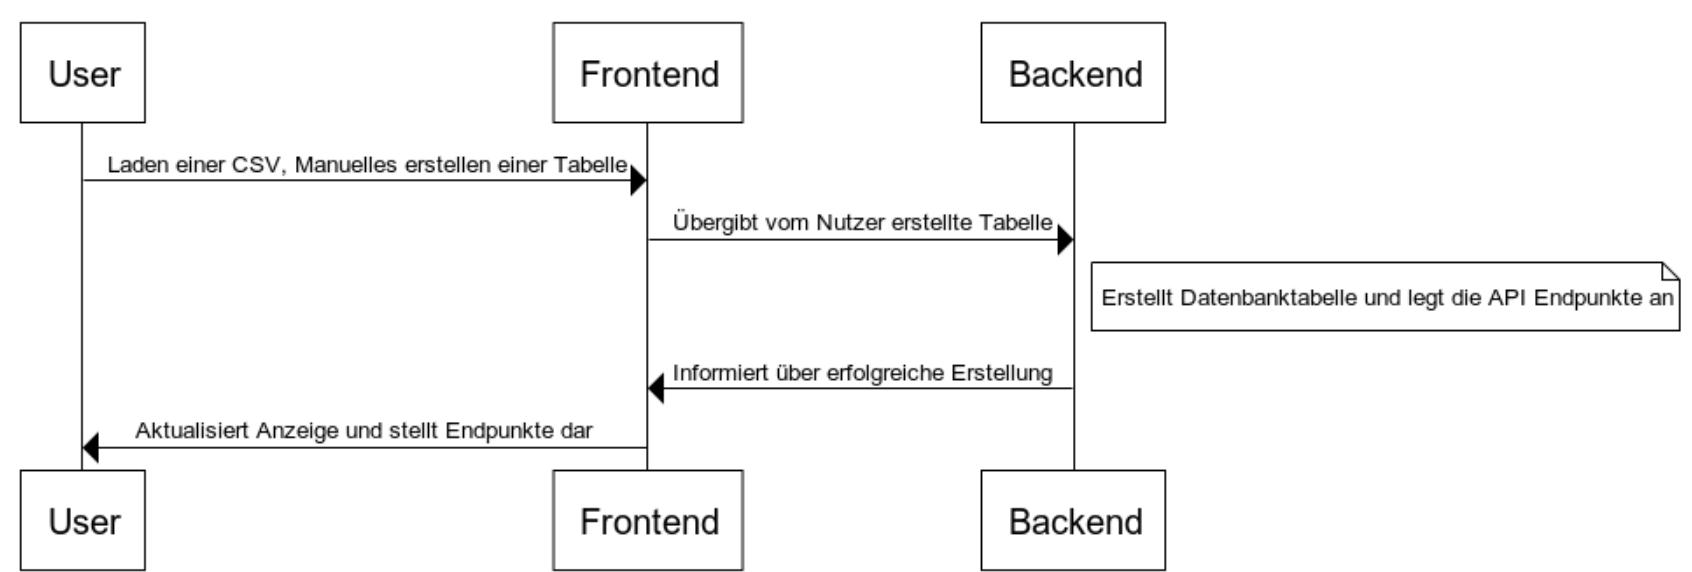
\includegraphics[width=1\textwidth]{figures/seq-hinzufuegen-von-ressourcen.png}
    \caption{Hinzufügen von Ressourcen}
    \label{fig:add-ressources}
\end{figure}
Das zweite Szenario bezieht sich auf die Abfrage einer Ressource. Zunächst wird hierbei eine \textit{GET}-Abfrage an den Server gestellt.
\begin{verbatim}
    GET http://localhost:3000/api/users?id=1
\end{verbatim}
Erwartungsgemäß sollte die Antwort des Servers ein \gls{json}-Objekt sein, welches die gespeicherten Daten des Users mit der ID 1 enthält. Nach dem Eingang der Anfrage prüft das Backend zunächst, ob die Ressource vorhanden ist. Ist dies nicht der Fall, antwortet der Server mit dem HTTP Status-Code \textit{404 NOT FOUND}. Dies indiziert das Nichtvorhandensein einer angefragten Ressource. Ist sie jedoch vorhanden, ruft der Server die zugrundeliegenden Daten aus der Datenbank ab und gibt eine entsprechende \gls{json}-formatierte Nachricht zurück. Darin enthalten sind mehrere Attribute. Der Status, eine Nachricht (message), in der auch eventuelle Fehlermeldungen an den Client zurückgegeben werden können und die eigentlichen Daten (data).
\begin{figure}[h]
    \centering
    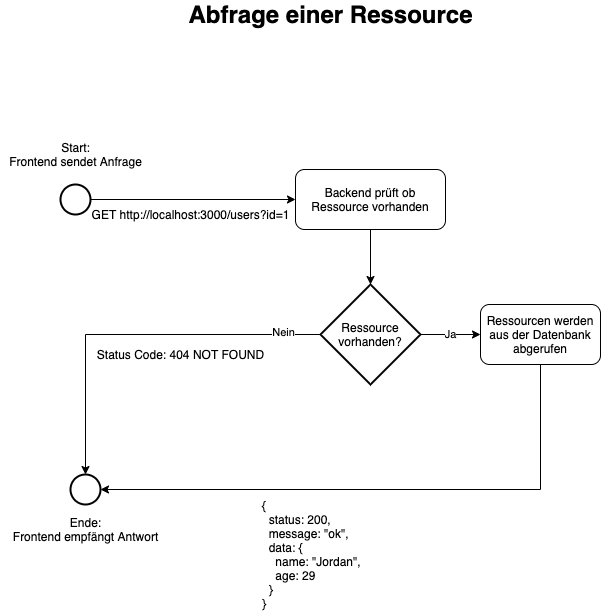
\includegraphics[width=0.8\textwidth]{figures/fc-abfrage-ressource.png}
    \caption{Abfrage einer Ressource}
    \label{fig:request-ressource}
\end{figure}
Daraus lässt sich also schließen, dass der Anwender auf der Konfigurationsoberfläche die Möglichkeit hat Daten entweder manuell in eine Tabelle einzutragen oder eine eigens erstellte \gls{csv}-Datei hochzuladen.
\\
Das Frontend muss mit dem Backend kommunizieren, um Tabellen anzulegen oder zu entfernen. Dies wird über eigene Endpunkte zur Administration geschehen. 

\begin{verbatim}
    PUT http://localhost:3000/api/admin/table
    DELETE http://localhost:3000/api/admin/table?name=users
\end{verbatim}
Über den \textit{PUT}-Request können Tabellen neu hinzugefügt oder überschrieben werden. Über den \textit{DELETE}-Request werden Tabellen hingegen gelöscht.
Ferner müssen Endpunkte zur Manipulation der Daten bereitgestellt werden. Da diese immer einheitlich sind, genügt es die Tabellennamen in einer Datenbank zu speichern und somit auf Validität der Endpunkte bei Abfragen zu prüfen.

\section{Architekturdesign} \label{sec:architecture}
Dieses Kapitel befasst sich zunächst mit dem groben Aufbau der Anwendung. Hierbei wird skizziert, wie Frontend, Backend und Datenbank in Relation zueinander stehen. Der zweite Teil dieses Kapitels befasst sich mit der verwendeten Technologie zur Programmierung des Frontends, Backends und der verwendeten Datenspeicherungsmethode.  

\begin{figure}[h]
    \centering
    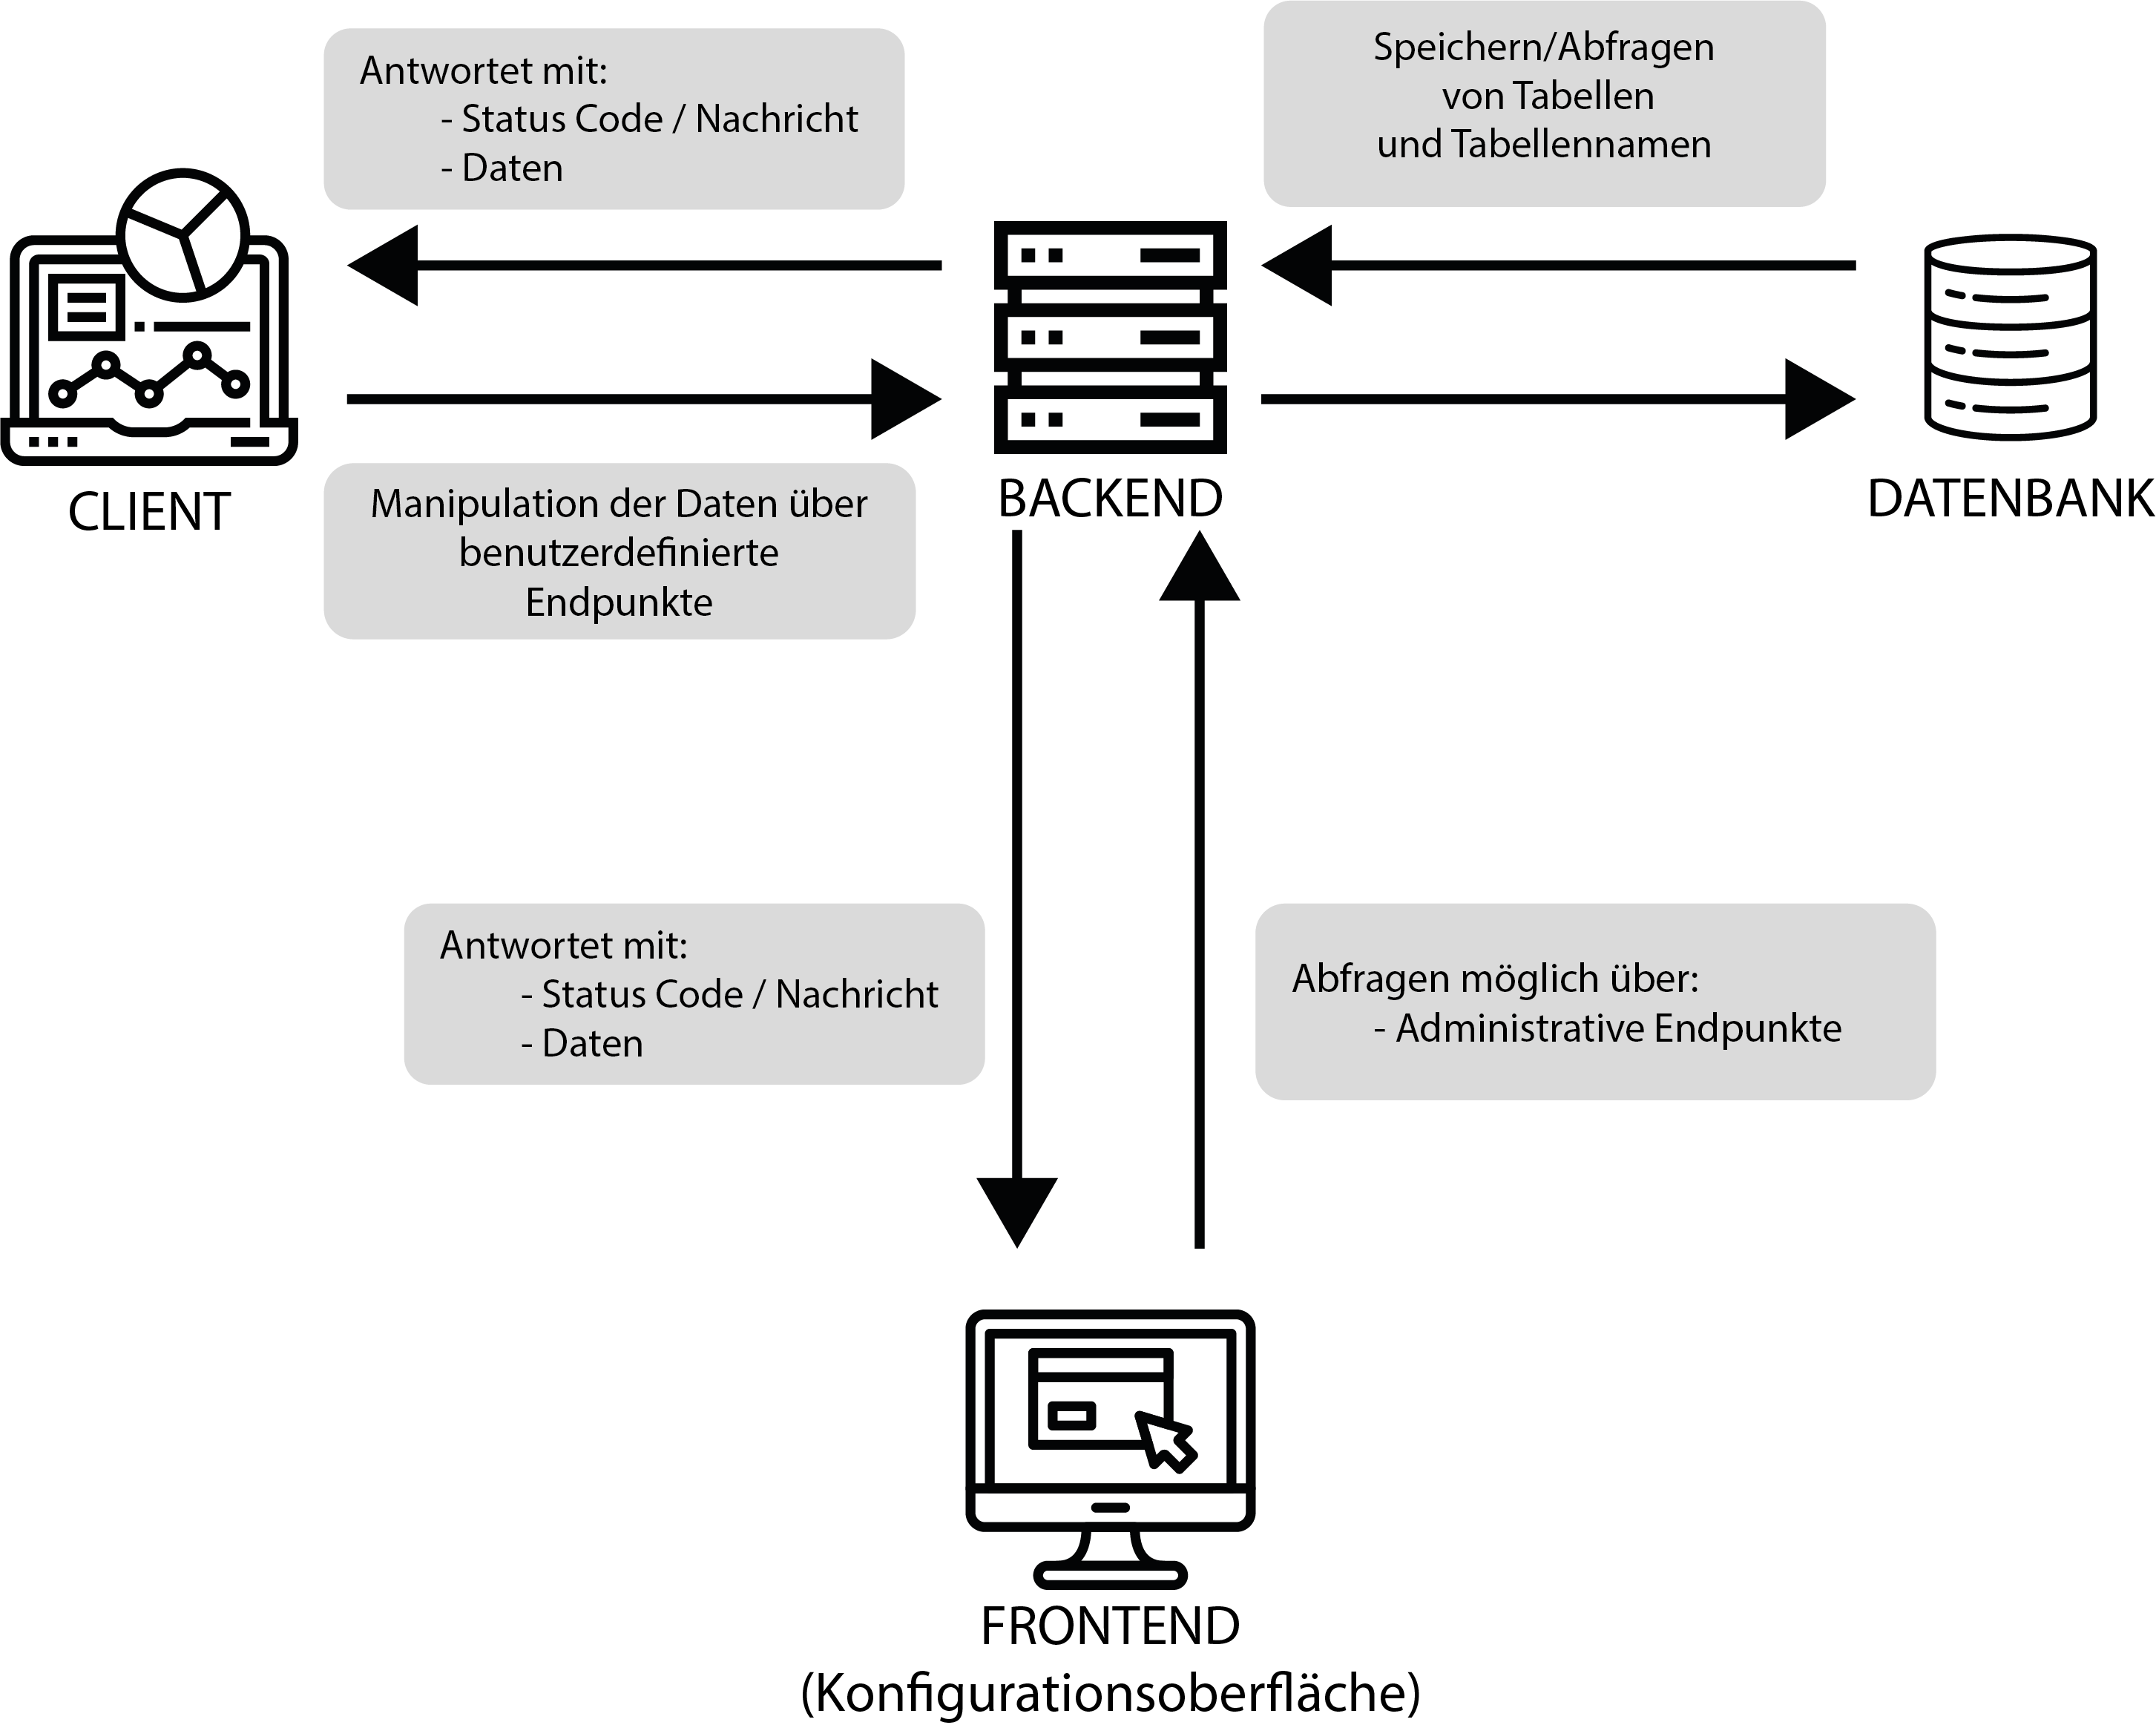
\includegraphics[width=0.8\textwidth]{figures/grobkonzept.png}
    \caption{Grobkonzept}
    \label{fig:grobkonzept}
\end{figure}

\subsubsection{Grober Entwurf}
Der erste Entwurf des Aufbaus (\autoref{fig:grobkonzept} - Icons von Flaticon\footnote{https://www.freepikcompany.com/legal}) ist in vier Teile unterteilt: Backend, Frontend, Client, Datenbank. Der Server (Backend) bildet dabei die zentrale Vermittlungsstelle. Hier werden eingehende Anfragen von der Konfigurationsoberfläche und dem Client (\gls{restapi} Nutzer) bearbeitet und beantwortet. Des Weiteren agiert der Server mit einer Datenbank, um neue Tabellen zu speichern, bestehende zu überschreiben oder zu löschen. 

\subsubsection{Verwendete Technologien}
Zur Entwicklung des gesamten Projekts müssen in diesem Abschnitt die richtigen Technologien ausgewählt werden. Dazu gehören zum Beispiel die Programmiersprachen des Frontends und des Backends. Um die persistente Datenspeicherung zu ermöglichen, wird auch eine geeignete Datenbank ausgewählt. \\
Klassische Lösungen basieren auf dem sogenannten \gls{lamp}-Stack. Hierbei müsste lokal ein Apache-Server\footnote{https://httpd.apache.org/} gestartet werden, welcher PHP-Dateien\footnote{https://www.php.net/manual/de/intro-whatis.php} bereitstellt. Diese wiederum können mit einer MySQL\footnote{https://dev.mysql.com/doc/refman/8.0/en/what-is-mysql.html} Datenbank kommunizieren und die benötigten Daten bereitstellen. Zur Gestaltung der Webseiten kommen \gls{html} und \gls{css} zum Einsatz. Während \gls{html} die reine Auszeichnungssprache ist und das Grundgerüst von Komponenten darstellt, welche innerhalb des Browsers erzeugt werden, ist letzteres eine Sprache, um die Komponenten in zum Beispiel Farbe und Form zu gestalten. Die funktionale Programmiersprache \textit{JavaScript} wird hier nur dazu verwendet, um Webseiten dynamischer zu gestalten. So ist beispielsweise das Auslesen von Eingabefeldern oder das Auswerten eines Knopfdrucks möglich \cite{Gerner.2006}. \\ \\ Die Programmiersprache JavaScript hat sich im laufe der Zeit sehr weit entwickelt und findet heutzutage auch außerhalb der Browserumgebung Verwendung. Die Sprache wird beispielsweise auch serverseitig eingesetzt und durch eine Laufzeitumgebung wie \textit{node.js}\footnote{https://nodejs.org/en/about/} für serverseitige Anwendungsszenarien eingesetzt. \cite{Resig.2016} Gleichzeitig ließe sich die Konfigurationsoberfläche ebenfalls mit node.js bereitstellen. Der Vorteil Front- und Backend in einer gemeinsamen Sprache zu programmieren legt nahe node.js für dieses Projekt einzusetzen. \\ Offen bleibt die Frage, wie Daten innerhalb des Systems persistiert werden. Wie bereits erwähnt, ist eine Möglichkeit die Nutzung einer relationalen \textit{MySQL} Datenbank. Jedoch wird hierfür ein weiterer ressourcen-intensiver Server benötigt \cite{Gerner.2006}. Für einen solchen, eher kleinen Datenbestand, lässt sich eine \textit{SQLite}-Datenbank in Betracht ziehen. Im Gegensatz zur herkömmlichen MySQL-Datenbank, werden Daten in einer Datei abgelegt und zur Laufzeit aus dieser gelesen respektive geschrieben. Trotz der serverlosen Datenbankarchitektur ermöglicht SQLite die meisten Features, welche MySQL bietet.\footnote{https://www.sqlite.org/about.html}

\subsubsection{Systemarchitektur} \label{subsub:system-architectuere}
Ein nicht von der Hand zu weisender Faktor bei der Entwicklung von Softwareprojekten, ist der zugrundeliegende Aufbau einer Software. Bei modernen Webanwendungen wird auf das sehr weit verbreitete \gls{mvc} Muster zurückgegriffen. Dabei wird das System in mehrere Schichten unterteilt, welche verschiedene Bereiche voneinander trennen. Bei einer in node.js geschriebenen \gls{restapi} sind das typischerweise:
\begin{itemize}
    \item Model: Datenmodell; Zugriff auf Datenbank (Lesen, Schreiben); Umwandlung in JS-Objekte
    \item Controller: Verarbeiten, validieren und beantworten der eingehenden \gls{http}-Anfragen.
    \item  Service: Business-Logik, hier ist der logische Programmcode implementiert
    \item Tests: Modultests, um einzelne Bereiche zu testen. 
    \item Sonstige: util - gemeinsame Funktionen; constants - gemeinsame Konstanten
\end{itemize}
In \autoref{fig:project-structure} ist der Aufbau des Projekts im Detail erkennbar. Der Ordner \textit{node{\_}modules} beinhaltet lediglich Module, welche von node.js genutzt werden. 
Die Konfigurationsoberfläche (View) ist ebenfalls in dieser Struktur, in Form des \textit{Public}-Ordners, vorhanden. Der Aufbau des Frontend-Ordners ist ebenfalls Modular unterteilt. So befindet sich \gls{css} in dem dafür angelegten Ordner. \textit{Assets}, also Bilddatein, Schriftarten oder sonstige Dateien, werden im gleichnamigen Ordner abgelegt. Die JavaScript-Dateien befinden sich ebenfalls in einem Unterordner. \\
Dank der Einführung von JavaScript-Modulen im Browser mit dem Standard \textit{ECMA-Script 2016} wird hier auch ein modularer Aufbau ermöglicht. Im Gegensatz zum normalen Webseiten Aufbau, kann in die Webseite ein einziges Modul importiert werden (\textit{main.js}), welches auf Funktionen in den einzelnen Untermodulen zugreift. Dies ermöglicht einen strukturierten und lesbareren Aufbau. \cite{Mozilla.2020}

\begin{figure}[h]
    \centering
    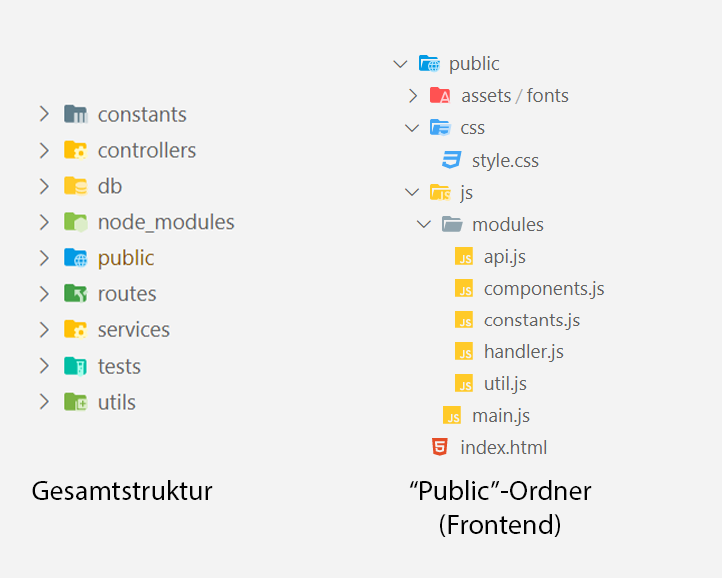
\includegraphics[width=0.6\textwidth]{figures/ordner-strukturen.png}
    \caption{Projektstruktur}
    \label{fig:project-structure}
\end{figure}
